\documentclass{report}

%%%%%%%%%%%%%%%%%%%%%%%%%%%%%%%%%
% PACKAGE IMPORTS
%%%%%%%%%%%%%%%%%%%%%%%%%%%%%%%%%


\usepackage[tmargin=2cm,rmargin=1in,lmargin=1in,margin=0.85in,bmargin=2cm,footskip=.2in]{geometry}
\usepackage{amsmath,amsfonts,amsthm,amssymb,mathtools}
\usepackage[varbb]{newpxmath}
\usepackage{xfrac}
\usepackage[makeroom]{cancel}
\usepackage{mathtools}
\usepackage{bookmark}
\usepackage{enumitem}
\usepackage{hyperref,theoremref}
\hypersetup{
	pdftitle={Assignment},
	colorlinks=true, linkcolor=doc!90,
	bookmarksnumbered=true,
	bookmarksopen=true
}
\usepackage[most,many,breakable]{tcolorbox}
\usepackage{xcolor}
\usepackage{varwidth}
\usepackage{varwidth}
\usepackage{etoolbox}
%\usepackage{authblk}
\usepackage{nameref}
\usepackage{multicol,array}
\usepackage{tikz-cd}
\usepackage[ruled,vlined,linesnumbered]{algorithm2e}
\usepackage{comment} % enables the use of multi-line comments (\ifx \fi) 
\usepackage{import}
\usepackage{xifthen}
\usepackage{pdfpages}
\usepackage{transparent}

% \usepackage{extsizes}

\newcommand\mycommfont[1]{\footnotesize\ttfamily\textcolor{blue}{#1}}
\SetCommentSty{mycommfont}
\newcommand{\incfig}[1]{%
    \def\svgwidth{\columnwidth}
    \import{./figures/}{#1.pdf_tex}
}

\usepackage{tikzsymbols}
\renewcommand\qedsymbol{$\Laughey$}


%\usepackage{import}
%\usepackage{xifthen}
%\usepackage{pdfpages}
%\usepackage{transparent}


%%%%%%%%%%%%%%%%%%%%%%%%%%%%%%
% SELF MADE COLORS
%%%%%%%%%%%%%%%%%%%%%%%%%%%%%%



\definecolor{myg}{RGB}{56, 140, 70}
\definecolor{myb}{RGB}{45, 111, 177}
\definecolor{myr}{RGB}{199, 68, 64}
\definecolor{mytheorembg}{HTML}{F2F2F9}
\definecolor{mytheoremfr}{HTML}{00007B}
\definecolor{mylenmabg}{HTML}{FFFAF8}
\definecolor{mylenmafr}{HTML}{983b0f}
\definecolor{mypropbg}{HTML}{f2fbfc}
\definecolor{mypropfr}{HTML}{191971}
\definecolor{myexamplebg}{HTML}{F2FBF8}
\definecolor{myexamplefr}{HTML}{88D6D1}
\definecolor{myexampleti}{HTML}{2A7F7F}
\definecolor{mydefinitbg}{HTML}{E5E5FF}
\definecolor{mydefinitfr}{HTML}{3F3FA3}
\definecolor{notesgreen}{RGB}{0,162,0}
\definecolor{myp}{RGB}{197, 92, 212}
\definecolor{mygr}{HTML}{2C3338}
\definecolor{myred}{RGB}{127,0,0}
\definecolor{myyellow}{RGB}{169,121,69}
\definecolor{myexercisebg}{HTML}{F2FBF8}
\definecolor{myexercisefg}{HTML}{88D6D1}


%%%%%%%%%%%%%%%%%%%%%%%%%%%%
% TCOLORBOX SETUPS
%%%%%%%%%%%%%%%%%%%%%%%%%%%%

\setlength{\parindent}{1cm}
%================================
% THEOREM BOX
%================================

\tcbuselibrary{theorems,skins,hooks}
\newtcbtheorem[number within=section]{Theorem}{Theorem}
{%
	enhanced,
	breakable,
	colback = mytheorembg,
	frame hidden,
	boxrule = 0sp,
	borderline west = {2pt}{0pt}{mytheoremfr},
	sharp corners,
	detach title,
	before upper = \tcbtitle\par\smallskip,
	coltitle = mytheoremfr,
	fonttitle = \bfseries\sffamily,
	description font = \mdseries,
	separator sign none,
	segmentation style={solid, mytheoremfr},
}
{th}

\tcbuselibrary{theorems,skins,hooks}
\newtcbtheorem[number within=chapter]{theorem}{Theorem}
{%
	enhanced,
	breakable,
	colback = mytheorembg,
	frame hidden,
	boxrule = 0sp,
	borderline west = {2pt}{0pt}{mytheoremfr},
	sharp corners,
	detach title,
	before upper = \tcbtitle\par\smallskip,
	coltitle = mytheoremfr,
	fonttitle = \bfseries\sffamily,
	description font = \mdseries,
	separator sign none,
	segmentation style={solid, mytheoremfr},
}
{th}


\tcbuselibrary{theorems,skins,hooks}
\newtcolorbox{Theoremcon}
{%
	enhanced
	,breakable
	,colback = mytheorembg
	,frame hidden
	,boxrule = 0sp
	,borderline west = {2pt}{0pt}{mytheoremfr}
	,sharp corners
	,description font = \mdseries
	,separator sign none
}

%================================
% Corollery
%================================
\tcbuselibrary{theorems,skins,hooks}
\newtcbtheorem[number within=section]{Corollary}{Corollary}
{%
	enhanced
	,breakable
	,colback = myp!10
	,frame hidden
	,boxrule = 0sp
	,borderline west = {2pt}{0pt}{myp!85!black}
	,sharp corners
	,detach title
	,before upper = \tcbtitle\par\smallskip
	,coltitle = myp!85!black
	,fonttitle = \bfseries\sffamily
	,description font = \mdseries
	,separator sign none
	,segmentation style={solid, myp!85!black}
}
{th}
\tcbuselibrary{theorems,skins,hooks}
\newtcbtheorem[number within=chapter]{corollary}{Corollary}
{%
	enhanced
	,breakable
	,colback = myp!10
	,frame hidden
	,boxrule = 0sp
	,borderline west = {2pt}{0pt}{myp!85!black}
	,sharp corners
	,detach title
	,before upper = \tcbtitle\par\smallskip
	,coltitle = myp!85!black
	,fonttitle = \bfseries\sffamily
	,description font = \mdseries
	,separator sign none
	,segmentation style={solid, myp!85!black}
}
{th}


%================================
% LENMA
%================================

\tcbuselibrary{theorems,skins,hooks}
\newtcbtheorem[number within=section]{Lenma}{Lenma}
{%
	enhanced,
	breakable,
	colback = mylenmabg,
	frame hidden,
	boxrule = 0sp,
	borderline west = {2pt}{0pt}{mylenmafr},
	sharp corners,
	detach title,
	before upper = \tcbtitle\par\smallskip,
	coltitle = mylenmafr,
	fonttitle = \bfseries\sffamily,
	description font = \mdseries,
	separator sign none,
	segmentation style={solid, mylenmafr},
}
{th}

\tcbuselibrary{theorems,skins,hooks}
\newtcbtheorem[number within=chapter]{lenma}{Lenma}
{%
	enhanced,
	breakable,
	colback = mylenmabg,
	frame hidden,
	boxrule = 0sp,
	borderline west = {2pt}{0pt}{mylenmafr},
	sharp corners,
	detach title,
	before upper = \tcbtitle\par\smallskip,
	coltitle = mylenmafr,
	fonttitle = \bfseries\sffamily,
	description font = \mdseries,
	separator sign none,
	segmentation style={solid, mylenmafr},
}
{th}


%================================
% PROPOSITION
%================================

\tcbuselibrary{theorems,skins,hooks}
\newtcbtheorem[number within=section]{Prop}{Proposition}
{%
	enhanced,
	breakable,
	colback = mypropbg,
	frame hidden,
	boxrule = 0sp,
	borderline west = {2pt}{0pt}{mypropfr},
	sharp corners,
	detach title,
	before upper = \tcbtitle\par\smallskip,
	coltitle = mypropfr,
	fonttitle = \bfseries\sffamily,
	description font = \mdseries,
	separator sign none,
	segmentation style={solid, mypropfr},
}
{th}

\tcbuselibrary{theorems,skins,hooks}
\newtcbtheorem[number within=chapter]{prop}{Proposition}
{%
	enhanced,
	breakable,
	colback = mypropbg,
	frame hidden,
	boxrule = 0sp,
	borderline west = {2pt}{0pt}{mypropfr},
	sharp corners,
	detach title,
	before upper = \tcbtitle\par\smallskip,
	coltitle = mypropfr,
	fonttitle = \bfseries\sffamily,
	description font = \mdseries,
	separator sign none,
	segmentation style={solid, mypropfr},
}
{th}


%================================
% CLAIM
%================================

\tcbuselibrary{theorems,skins,hooks}
\newtcbtheorem[number within=section]{claim}{Claim}
{%
	enhanced
	,breakable
	,colback = myg!10
	,frame hidden
	,boxrule = 0sp
	,borderline west = {2pt}{0pt}{myg}
	,sharp corners
	,detach title
	,before upper = \tcbtitle\par\smallskip
	,coltitle = myg!85!black
	,fonttitle = \bfseries\sffamily
	,description font = \mdseries
	,separator sign none
	,segmentation style={solid, myg!85!black}
}
{th}



%================================
% Exercise
%================================

\tcbuselibrary{theorems,skins,hooks}
\newtcbtheorem[number within=section]{Exercise}{Exercise}
{%
	enhanced,
	breakable,
	colback = myexercisebg,
	frame hidden,
	boxrule = 0sp,
	borderline west = {2pt}{0pt}{myexercisefg},
	sharp corners,
	detach title,
	before upper = \tcbtitle\par\smallskip,
	coltitle = myexercisefg,
	fonttitle = \bfseries\sffamily,
	description font = \mdseries,
	separator sign none,
	segmentation style={solid, myexercisefg},
}
{th}

\tcbuselibrary{theorems,skins,hooks}
\newtcbtheorem[number within=chapter]{exercise}{Exercise}
{%
	enhanced,
	breakable,
	colback = myexercisebg,
	frame hidden,
	boxrule = 0sp,
	borderline west = {2pt}{0pt}{myexercisefg},
	sharp corners,
	detach title,
	before upper = \tcbtitle\par\smallskip,
	coltitle = myexercisefg,
	fonttitle = \bfseries\sffamily,
	description font = \mdseries,
	separator sign none,
	segmentation style={solid, myexercisefg},
}
{th}

%================================
% EXAMPLE BOX
%================================

\newtcbtheorem[number within=section]{Example}{Example}
{%
	colback = myexamplebg
	,breakable
	,colframe = myexamplefr
	,coltitle = myexampleti
	,boxrule = 1pt
	,sharp corners
	,detach title
	,before upper=\tcbtitle\par\smallskip
	,fonttitle = \bfseries
	,description font = \mdseries
	,separator sign none
	,description delimiters parenthesis
}
{ex}

\newtcbtheorem[number within=chapter]{example}{Example}
{%
	colback = myexamplebg
	,breakable
	,colframe = myexamplefr
	,coltitle = myexampleti
	,boxrule = 1pt
	,sharp corners
	,detach title
	,before upper=\tcbtitle\par\smallskip
	,fonttitle = \bfseries
	,description font = \mdseries
	,separator sign none
	,description delimiters parenthesis
}
{ex}

%================================
% DEFINITION BOX
%================================

\newtcbtheorem[number within=section]{Definition}{Definition}{enhanced,
	before skip=2mm,after skip=2mm, colback=red!5,colframe=red!80!black,boxrule=0.5mm,
	attach boxed title to top left={xshift=1cm,yshift*=1mm-\tcboxedtitleheight}, varwidth boxed title*=-3cm,
	boxed title style={frame code={
					\path[fill=tcbcolback]
					([yshift=-1mm,xshift=-1mm]frame.north west)
					arc[start angle=0,end angle=180,radius=1mm]
					([yshift=-1mm,xshift=1mm]frame.north east)
					arc[start angle=180,end angle=0,radius=1mm];
					\path[left color=tcbcolback!60!black,right color=tcbcolback!60!black,
						middle color=tcbcolback!80!black]
					([xshift=-2mm]frame.north west) -- ([xshift=2mm]frame.north east)
					[rounded corners=1mm]-- ([xshift=1mm,yshift=-1mm]frame.north east)
					-- (frame.south east) -- (frame.south west)
					-- ([xshift=-1mm,yshift=-1mm]frame.north west)
					[sharp corners]-- cycle;
				},interior engine=empty,
		},
	fonttitle=\bfseries,
	title={#2},#1}{def}
\newtcbtheorem[number within=chapter]{definition}{Definition}{enhanced,
	before skip=2mm,after skip=2mm, colback=red!5,colframe=red!80!black,boxrule=0.5mm,
	attach boxed title to top left={xshift=1cm,yshift*=1mm-\tcboxedtitleheight}, varwidth boxed title*=-3cm,
	boxed title style={frame code={
					\path[fill=tcbcolback]
					([yshift=-1mm,xshift=-1mm]frame.north west)
					arc[start angle=0,end angle=180,radius=1mm]
					([yshift=-1mm,xshift=1mm]frame.north east)
					arc[start angle=180,end angle=0,radius=1mm];
					\path[left color=tcbcolback!60!black,right color=tcbcolback!60!black,
						middle color=tcbcolback!80!black]
					([xshift=-2mm]frame.north west) -- ([xshift=2mm]frame.north east)
					[rounded corners=1mm]-- ([xshift=1mm,yshift=-1mm]frame.north east)
					-- (frame.south east) -- (frame.south west)
					-- ([xshift=-1mm,yshift=-1mm]frame.north west)
					[sharp corners]-- cycle;
				},interior engine=empty,
		},
	fonttitle=\bfseries,
	title={#2},#1}{def}



%================================
% Solution BOX
%================================

\makeatletter
\newtcbtheorem{question}{Question}{enhanced,
	breakable,
	colback=white,
	colframe=myb!80!black,
	attach boxed title to top left={yshift*=-\tcboxedtitleheight},
	fonttitle=\bfseries,
	title={#2},
	boxed title size=title,
	boxed title style={%
			sharp corners,
			rounded corners=northwest,
			colback=tcbcolframe,
			boxrule=0pt,
		},
	underlay boxed title={%
			\path[fill=tcbcolframe] (title.south west)--(title.south east)
			to[out=0, in=180] ([xshift=5mm]title.east)--
			(title.center-|frame.east)
			[rounded corners=\kvtcb@arc] |-
			(frame.north) -| cycle;
		},
	#1
}{def}
\makeatother

%================================
% SOLUTION BOX
%================================

\makeatletter
\newtcolorbox{solution}{enhanced,
	breakable,
	colback=white,
	colframe=myg!80!black,
	attach boxed title to top left={yshift*=-\tcboxedtitleheight},
	title=Solution,
	boxed title size=title,
	boxed title style={%
			sharp corners,
			rounded corners=northwest,
			colback=tcbcolframe,
			boxrule=0pt,
		},
	underlay boxed title={%
			\path[fill=tcbcolframe] (title.south west)--(title.south east)
			to[out=0, in=180] ([xshift=5mm]title.east)--
			(title.center-|frame.east)
			[rounded corners=\kvtcb@arc] |-
			(frame.north) -| cycle;
		},
}
\makeatother

%================================
% Question BOX
%================================

\makeatletter
\newtcbtheorem{qstion}{Question}{enhanced,
	breakable,
	colback=white,
	colframe=mygr,
	attach boxed title to top left={yshift*=-\tcboxedtitleheight},
	fonttitle=\bfseries,
	title={#2},
	boxed title size=title,
	boxed title style={%
			sharp corners,
			rounded corners=northwest,
			colback=tcbcolframe,
			boxrule=0pt,
		},
	underlay boxed title={%
			\path[fill=tcbcolframe] (title.south west)--(title.south east)
			to[out=0, in=180] ([xshift=5mm]title.east)--
			(title.center-|frame.east)
			[rounded corners=\kvtcb@arc] |-
			(frame.north) -| cycle;
		},
	#1
}{def}
\makeatother

\newtcbtheorem[number within=chapter]{wconc}{Wrong Concept}{
	breakable,
	enhanced,
	colback=white,
	colframe=myr,
	arc=0pt,
	outer arc=0pt,
	fonttitle=\bfseries\sffamily\large,
	colbacktitle=myr,
	attach boxed title to top left={},
	boxed title style={
			enhanced,
			skin=enhancedfirst jigsaw,
			arc=3pt,
			bottom=0pt,
			interior style={fill=myr}
		},
	#1
}{def}



%================================
% NOTE BOX
%================================

\usetikzlibrary{arrows,calc,shadows.blur}
\tcbuselibrary{skins}
\newtcolorbox{note}[1][]{%
	enhanced jigsaw,
	colback=gray!20!white,%
	colframe=gray!80!black,
	size=small,
	boxrule=1pt,
	title=\textbf{Note:},
	halign title=flush center,
	coltitle=black,
	breakable,
	drop shadow=black!50!white,
	attach boxed title to top left={xshift=1cm,yshift=-\tcboxedtitleheight/2,yshifttext=-\tcboxedtitleheight/2},
	minipage boxed title=1.5cm,
	boxed title style={%
			colback=white,
			size=fbox,
			boxrule=1pt,
			boxsep=2pt,
			underlay={%
					\coordinate (dotA) at ($(interior.west) + (-0.5pt,0)$);
					\coordinate (dotB) at ($(interior.east) + (0.5pt,0)$);
					\begin{scope}
						\clip (interior.north west) rectangle ([xshift=3ex]interior.east);
						\filldraw [white, blur shadow={shadow opacity=60, shadow yshift=-.75ex}, rounded corners=2pt] (interior.north west) rectangle (interior.south east);
					\end{scope}
					\begin{scope}[gray!80!black]
						\fill (dotA) circle (2pt);
						\fill (dotB) circle (2pt);
					\end{scope}
				},
		},
	#1,
}

%%%%%%%%%%%%%%%%%%%%%%%%%%%%%%
% SELF MADE COMMANDS
%%%%%%%%%%%%%%%%%%%%%%%%%%%%%%


\newcommand{\thm}[2]{\begin{Theorem}{#1}{}#2\end{Theorem}}
\newcommand{\cor}[2]{\begin{Corollary}{#1}{}#2\end{Corollary}}
\newcommand{\mlenma}[2]{\begin{Lenma}{#1}{}#2\end{Lenma}}
\newcommand{\mprop}[2]{\begin{Prop}{#1}{}#2\end{Prop}}
\newcommand{\clm}[3]{\begin{claim}{#1}{#2}#3\end{claim}}
\newcommand{\wc}[2]{\begin{wconc}{#1}{}\setlength{\parindent}{1cm}#2\end{wconc}}
\newcommand{\thmcon}[1]{\begin{Theoremcon}{#1}\end{Theoremcon}}
\newcommand{\ex}[2]{\begin{Example}{#1}{}#2\end{Example}}
\newcommand{\dfn}[2]{\begin{Definition}[colbacktitle=red!75!black]{#1}{}#2\end{Definition}}
\newcommand{\dfnc}[2]{\begin{definition}[colbacktitle=red!75!black]{#1}{}#2\end{definition}}
\newcommand{\qs}[2]{\begin{question*}{#1}{}#2\end{question*}}
\newcommand{\mpf}[2]{\begin{myproof}[#1]#2\end{myproof}}
\newcommand{\nt}[1]{\begin{note}#1\end{note}}

\newcommand*\circled[1]{\tikz[baseline=(char.base)]{
		\node[shape=circle,draw,inner sep=1pt] (char) {#1};}}
\newcommand\getcurrentref[1]{%
	\ifnumequal{\value{#1}}{0}
	{??}
	{\the\value{#1}}%
}
\newcommand{\getCurrentSectionNumber}{\getcurrentref{section}}
\newenvironment{myproof}[1][\proofname]{%
	\proof[\bfseries #1: ]%
}{\endproof}

\newcommand{\mclm}[2]{\begin{myclaim}[#1]#2\end{myclaim}}
\newenvironment{myclaim}[1][\claimname]{\proof[\bfseries #1: ]}{}

\newcounter{mylabelcounter}

\makeatletter
\newcommand{\setword}[2]{%
	\phantomsection
	#1\def\@currentlabel{\unexpanded{#1}}\label{#2}%
}
\makeatother




\tikzset{
	symbol/.style={
			draw=none,
			every to/.append style={
					edge node={node [sloped, allow upside down, auto=false]{$#1$}}}
		}
}


% deliminators
\DeclarePairedDelimiter{\abs}{\lvert}{\rvert}
\DeclarePairedDelimiter{\norm}{\lVert}{\rVert}

\DeclarePairedDelimiter{\ceil}{\lceil}{\rceil}
\DeclarePairedDelimiter{\floor}{\lfloor}{\rfloor}
\DeclarePairedDelimiter{\round}{\lfloor}{\rceil}

\newsavebox\diffdbox
\newcommand{\slantedromand}{{\mathpalette\makesl{d}}}
\newcommand{\makesl}[2]{%
\begingroup
\sbox{\diffdbox}{$\mathsurround=0pt#1\mathrm{#2}$}%
\pdfsave
\pdfsetmatrix{1 0 0.2 1}%
\rlap{\usebox{\diffdbox}}%
\pdfrestore
\hskip\wd\diffdbox
\endgroup
}
\newcommand{\dd}[1][]{\ensuremath{\mathop{}\!\ifstrempty{#1}{%
\slantedromand\@ifnextchar^{\hspace{0.2ex}}{\hspace{0.1ex}}}%
{\slantedromand\hspace{0.2ex}^{#1}}}}
\ProvideDocumentCommand\dv{o m g}{%
  \ensuremath{%
    \IfValueTF{#3}{%
      \IfNoValueTF{#1}{%
        \frac{\dd #2}{\dd #3}%
      }{%
        \frac{\dd^{#1} #2}{\dd #3^{#1}}%
      }%
    }{%
      \IfNoValueTF{#1}{%
        \frac{\dd}{\dd #2}%
      }{%
        \frac{\dd^{#1}}{\dd #2^{#1}}%
      }%
    }%
  }%
}
\providecommand*{\pdv}[3][]{\frac{\partial^{#1}#2}{\partial#3^{#1}}}
%  - others
\DeclareMathOperator{\Lap}{\mathcal{L}}
\DeclareMathOperator{\Var}{Var} % varience
\DeclareMathOperator{\Cov}{Cov} % covarience
\DeclareMathOperator{\E}{E} % expected

% Since the amsthm package isn't loaded

% I prefer the slanted \leq
\let\oldleq\leq % save them in case they're every wanted
\let\oldgeq\geq
\renewcommand{\leq}{\leqslant}
\renewcommand{\geq}{\geqslant}

% % redefine matrix env to allow for alignment, use r as default
% \renewcommand*\env@matrix[1][r]{\hskip -\arraycolsep
%     \let\@ifnextchar\new@ifnextchar
%     \array{*\c@MaxMatrixCols #1}}


%\usepackage{framed}
%\usepackage{titletoc}
%\usepackage{etoolbox}
%\usepackage{lmodern}


%\patchcmd{\tableofcontents}{\contentsname}{\sffamily\contentsname}{}{}

%\renewenvironment{leftbar}
%{\def\FrameCommand{\hspace{6em}%
%		{\color{myyellow}\vrule width 2pt depth 6pt}\hspace{1em}}%
%	\MakeFramed{\parshape 1 0cm \dimexpr\textwidth-6em\relax\FrameRestore}\vskip2pt%
%}
%{\endMakeFramed}

%\titlecontents{chapter}
%[0em]{\vspace*{2\baselineskip}}
%{\parbox{4.5em}{%
%		\hfill\Huge\sffamily\bfseries\color{myred}\thecontentspage}%
%	\vspace*{-2.3\baselineskip}\leftbar\textsc{\small\chaptername~\thecontentslabel}\\\sffamily}
%{}{\endleftbar}
%\titlecontents{section}
%[8.4em]
%{\sffamily\contentslabel{3em}}{}{}
%{\hspace{0.5em}\nobreak\itshape\color{myred}\contentspage}
%\titlecontents{subsection}
%[8.4em]
%{\sffamily\contentslabel{3em}}{}{}  
%{\hspace{0.5em}\nobreak\itshape\color{myred}\contentspage}



%%%%%%%%%%%%%%%%%%%%%%%%%%%%%%%%%%%%%%%%%%%
% TABLE OF CONTENTS
%%%%%%%%%%%%%%%%%%%%%%%%%%%%%%%%%%%%%%%%%%%

\usepackage{tikz}
\definecolor{doc}{RGB}{0,60,110}
\usepackage{titletoc}
\contentsmargin{0cm}
\titlecontents{chapter}[3.7pc]
{\addvspace{30pt}%
	\begin{tikzpicture}[remember picture, overlay]%
		\draw[fill=doc!60,draw=doc!60] (-7,-.1) rectangle (-0.9,.5);%
		\pgftext[left,x=-3.5cm,y=0.2cm]{\color{white}\Large\sc\bfseries Chapter\ \thecontentslabel};%
	\end{tikzpicture}\color{doc!60}\large\sc\bfseries}%
{}
{}
{\;\titlerule\;\large\sc\bfseries Page \thecontentspage
	\begin{tikzpicture}[remember picture, overlay]
		\draw[fill=doc!60,draw=doc!60] (2pt,0) rectangle (4,0.1pt);
	\end{tikzpicture}}%
\titlecontents{section}[3.7pc]
{\addvspace{2pt}}
{\contentslabel[\thecontentslabel]{2pc}}
{}
{\hfill\small \thecontentspage}
[]
\titlecontents*{subsection}[3.7pc]
{\addvspace{-1pt}\small}
{}
{}
{\ --- \small\thecontentspage}
[ \textbullet\ ][]

\makeatletter
\renewcommand{\tableofcontents}{%
	\chapter*{%
	  \vspace*{-20\p@}%
	  \begin{tikzpicture}[remember picture, overlay]%
		  \pgftext[right,x=15cm,y=0.2cm]{\color{doc!60}\Huge\sc\bfseries \contentsname};%
		  \draw[fill=doc!60,draw=doc!60] (13,-.75) rectangle (20,1);%
		  \clip (13,-.75) rectangle (20,1);
		  \pgftext[right,x=15cm,y=0.2cm]{\color{white}\Huge\sc\bfseries \contentsname};%
	  \end{tikzpicture}}%
	\@starttoc{toc}}
\makeatother
\newcommand{\id}{\mathrm{id}}
\newcommand{\taking}[1]{\xrightarrow{#1}}
\newcommand{\inv}{^{-1}}

%From M170 "Introduction to Graph Theory" at SJSU
\DeclareMathOperator{\diam}{diam}
\DeclareMathOperator{\ord}{ord}
\newcommand{\defeq}{\overset{\mathrm{def}}{=}}

%From the USAMO .tex files
\newcommand{\ts}{\textsuperscript}
\newcommand{\dg}{^\circ}
\newcommand{\ii}{\item}

% % From Math 55 and Math 145 at Harvard
% \newenvironment{subproof}[1][Proof]{%
% \begin{proof}[#1] \renewcommand{\qedsymbol}{$\blacksquare$}}%
% {\end{proof}}

\newcommand{\liff}{\leftrightarrow}
\newcommand{\lthen}{\rightarrow}
\newcommand{\opname}{\operatorname}
\newcommand{\surjto}{\twoheadrightarrow}
\newcommand{\injto}{\hookrightarrow}
\newcommand{\On}{\mathrm{On}} % ordinals
\DeclareMathOperator{\img}{im} % Image
\DeclareMathOperator{\Img}{Im} % Image
\DeclareMathOperator{\coker}{coker} % Cokernel
\DeclareMathOperator{\Coker}{Coker} % Cokernel
\DeclareMathOperator{\Ker}{Ker} % Kernel
\DeclareMathOperator{\rank}{rank}
\DeclareMathOperator{\Spec}{Spec} % spectrum
\DeclareMathOperator{\Tr}{Tr} % trace
\DeclareMathOperator{\pr}{pr} % projection
\DeclareMathOperator{\ext}{ext} % extension
\DeclareMathOperator{\pred}{pred} % predecessor
\DeclareMathOperator{\dom}{dom} % domain
\DeclareMathOperator{\ran}{ran} % range
\DeclareMathOperator{\Hom}{Hom} % homomorphism
\DeclareMathOperator{\Mor}{Mor} % morphisms
\DeclareMathOperator{\End}{End} % endomorphism

\newcommand{\eps}{\epsilon}
\newcommand{\veps}{\varepsilon}
\newcommand{\ol}{\overline}
\newcommand{\ul}{\underline}
\newcommand{\wt}{\widetilde}
\newcommand{\wh}{\widehat}
\newcommand{\vocab}[1]{\textbf{\color{blue} #1}}
\providecommand{\half}{\frac{1}{2}}
\newcommand{\dang}{\measuredangle} %% Directed angle
\newcommand{\ray}[1]{\overrightarrow{#1}}
\newcommand{\seg}[1]{\overline{#1}}
\newcommand{\arc}[1]{\wideparen{#1}}
\DeclareMathOperator{\cis}{cis}
\DeclareMathOperator*{\lcm}{lcm}
\DeclareMathOperator*{\argmin}{arg min}
\DeclareMathOperator*{\argmax}{arg max}
\newcommand{\cycsum}{\sum_{\mathrm{cyc}}}
\newcommand{\symsum}{\sum_{\mathrm{sym}}}
\newcommand{\cycprod}{\prod_{\mathrm{cyc}}}
\newcommand{\symprod}{\prod_{\mathrm{sym}}}
\newcommand{\Qed}{\begin{flushright}\qed\end{flushright}}
\newcommand{\parinn}{\setlength{\parindent}{1cm}}
\newcommand{\parinf}{\setlength{\parindent}{0cm}}
% \newcommand{\norm}{\|\cdot\|}
\newcommand{\inorm}{\norm_{\infty}}
\newcommand{\opensets}{\{V_{\alpha}\}_{\alpha\in I}}
\newcommand{\oset}{V_{\alpha}}
\newcommand{\opset}[1]{V_{\alpha_{#1}}}
\newcommand{\lub}{\text{lub}}
\newcommand{\del}[2]{\frac{\partial #1}{\partial #2}}
\newcommand{\Del}[3]{\frac{\partial^{#1} #2}{\partial^{#1} #3}}
\newcommand{\deld}[2]{\dfrac{\partial #1}{\partial #2}}
\newcommand{\Deld}[3]{\dfrac{\partial^{#1} #2}{\partial^{#1} #3}}
\newcommand{\lm}{\lambda}
\newcommand{\uin}{\mathbin{\rotatebox[origin=c]{90}{$\in$}}}
\newcommand{\usubset}{\mathbin{\rotatebox[origin=c]{90}{$\subset$}}}
\newcommand{\lt}{\left}
\newcommand{\rt}{\right}
\newcommand{\bs}[1]{\boldsymbol{#1}}
\newcommand{\exs}{\exists}
\newcommand{\st}{\strut}
\newcommand{\dps}[1]{\displaystyle{#1}}

\newcommand{\sol}{\setlength{\parindent}{0cm}\textbf{\textit{Solution:}}\setlength{\parindent}{1cm} }
\newcommand{\solve}[1]{\setlength{\parindent}{0cm}\textbf{\textit{Solution: }}\setlength{\parindent}{1cm}#1 \Qed}
% Things Lie
\newcommand{\kb}{\mathfrak b}
\newcommand{\kg}{\mathfrak g}
\newcommand{\kh}{\mathfrak h}
\newcommand{\kn}{\mathfrak n}
\newcommand{\ku}{\mathfrak u}
\newcommand{\kz}{\mathfrak z}
\DeclareMathOperator{\Ext}{Ext} % Ext functor
\DeclareMathOperator{\Tor}{Tor} % Tor functor
\newcommand{\gl}{\opname{\mathfrak{gl}}} % frak gl group
\renewcommand{\sl}{\opname{\mathfrak{sl}}} % frak sl group chktex 6

% More script letters etc.
\newcommand{\SA}{\mathcal A}
\newcommand{\SB}{\mathcal B}
\newcommand{\SC}{\mathcal C}
\newcommand{\SF}{\mathcal F}
\newcommand{\SG}{\mathcal G}
\newcommand{\SH}{\mathcal H}
\newcommand{\OO}{\mathcal O}

\newcommand{\SCA}{\mathscr A}
\newcommand{\SCB}{\mathscr B}
\newcommand{\SCC}{\mathscr C}
\newcommand{\SCD}{\mathscr D}
\newcommand{\SCE}{\mathscr E}
\newcommand{\SCF}{\mathscr F}
\newcommand{\SCG}{\mathscr G}
\newcommand{\SCH}{\mathscr H}

% Mathfrak primes
\newcommand{\km}{\mathfrak m}
\newcommand{\kp}{\mathfrak p}
\newcommand{\kq}{\mathfrak q}

% number sets
\newcommand{\RR}[1][]{\ensuremath{\ifstrempty{#1}{\mathbb{R}}{\mathbb{R}^{#1}}}}
\newcommand{\NN}[1][]{\ensuremath{\ifstrempty{#1}{\mathbb{N}}{\mathbb{N}^{#1}}}}
\newcommand{\ZZ}[1][]{\ensuremath{\ifstrempty{#1}{\mathbb{Z}}{\mathbb{Z}^{#1}}}}
\newcommand{\QQ}[1][]{\ensuremath{\ifstrempty{#1}{\mathbb{Q}}{\mathbb{Q}^{#1}}}}
\newcommand{\CC}[1][]{\ensuremath{\ifstrempty{#1}{\mathbb{C}}{\mathbb{C}^{#1}}}}
\newcommand{\PP}[1][]{\ensuremath{\ifstrempty{#1}{\mathbb{P}}{\mathbb{P}^{#1}}}}
\newcommand{\HH}[1][]{\ensuremath{\ifstrempty{#1}{\mathbb{H}}{\mathbb{H}^{#1}}}}
\newcommand{\FF}[1][]{\ensuremath{\ifstrempty{#1}{\mathbb{F}}{\mathbb{F}^{#1}}}}

% number sets without arguments
\newcommand{\R}{\ensuremath{\mathbb{R}}}
\newcommand{\N}{\ensuremath{\mathbb{N}}}
\newcommand{\Z}{\ensuremath{\mathbb{Z}}}
\newcommand{\Q}{\ensuremath{\mathbb{Q}}}
\newcommand{\C}{\ensuremath{\mathbb{C}}}
\newcommand{\F}{\ensuremath{\mathbb{F}}}

% expected value
\newcommand{\EE}{\ensuremath{\mathbb{E}}}
\newcommand{\charin}{\text{ char }}
\DeclareMathOperator{\sign}{sign}
\DeclareMathOperator{\Aut}{Aut}
\DeclareMathOperator{\Inn}{Inn}
\DeclareMathOperator{\Syl}{Syl}
\DeclareMathOperator{\Gal}{Gal}
\DeclareMathOperator{\GL}{GL} % General linear group
\DeclareMathOperator{\SL}{SL} % Special linear group

%---------------------------------------
% BlackBoard Math Fonts :-
%---------------------------------------

%Captital Letters
\newcommand{\bbA}{\mathbb{A}}	\newcommand{\bbB}{\mathbb{B}}
\newcommand{\bbC}{\mathbb{C}}	\newcommand{\bbD}{\mathbb{D}}
\newcommand{\bbE}{\mathbb{E}}	\newcommand{\bbF}{\mathbb{F}}
\newcommand{\bbG}{\mathbb{G}}	\newcommand{\bbH}{\mathbb{H}}
\newcommand{\bbI}{\mathbb{I}}	\newcommand{\bbJ}{\mathbb{J}}
\newcommand{\bbK}{\mathbb{K}}	\newcommand{\bbL}{\mathbb{L}}
\newcommand{\bbM}{\mathbb{M}}	\newcommand{\bbN}{\mathbb{N}}
\newcommand{\bbO}{\mathbb{O}}	\newcommand{\bbP}{\mathbb{P}}
\newcommand{\bbQ}{\mathbb{Q}}	\newcommand{\bbR}{\mathbb{R}}
\newcommand{\bbS}{\mathbb{S}}	\newcommand{\bbT}{\mathbb{T}}
\newcommand{\bbU}{\mathbb{U}}	\newcommand{\bbV}{\mathbb{V}}
\newcommand{\bbW}{\mathbb{W}}	\newcommand{\bbX}{\mathbb{X}}
\newcommand{\bbY}{\mathbb{Y}}	\newcommand{\bbZ}{\mathbb{Z}}

%---------------------------------------
% MathCal Fonts :-
%---------------------------------------

%Captital Letters
\newcommand{\mcA}{\mathcal{A}}	\newcommand{\mcB}{\mathcal{B}}
\newcommand{\mcC}{\mathcal{C}}	\newcommand{\mcD}{\mathcal{D}}
\newcommand{\mcE}{\mathcal{E}}	\newcommand{\mcF}{\mathcal{F}}
\newcommand{\mcG}{\mathcal{G}}	\newcommand{\mcH}{\mathcal{H}}
\newcommand{\mcI}{\mathcal{I}}	\newcommand{\mcJ}{\mathcal{J}}
\newcommand{\mcK}{\mathcal{K}}	\newcommand{\mcL}{\mathcal{L}}
\newcommand{\mcM}{\mathcal{M}}	\newcommand{\mcN}{\mathcal{N}}
\newcommand{\mcO}{\mathcal{O}}	\newcommand{\mcP}{\mathcal{P}}
\newcommand{\mcQ}{\mathcal{Q}}	\newcommand{\mcR}{\mathcal{R}}
\newcommand{\mcS}{\mathcal{S}}	\newcommand{\mcT}{\mathcal{T}}
\newcommand{\mcU}{\mathcal{U}}	\newcommand{\mcV}{\mathcal{V}}
\newcommand{\mcW}{\mathcal{W}}	\newcommand{\mcX}{\mathcal{X}}
\newcommand{\mcY}{\mathcal{Y}}	\newcommand{\mcZ}{\mathcal{Z}}


%---------------------------------------
% Bold Math Fonts :-
%---------------------------------------

%Captital Letters
\newcommand{\bmA}{\boldsymbol{A}}	\newcommand{\bmB}{\boldsymbol{B}}
\newcommand{\bmC}{\boldsymbol{C}}	\newcommand{\bmD}{\boldsymbol{D}}
\newcommand{\bmE}{\boldsymbol{E}}	\newcommand{\bmF}{\boldsymbol{F}}
\newcommand{\bmG}{\boldsymbol{G}}	\newcommand{\bmH}{\boldsymbol{H}}
\newcommand{\bmI}{\boldsymbol{I}}	\newcommand{\bmJ}{\boldsymbol{J}}
\newcommand{\bmK}{\boldsymbol{K}}	\newcommand{\bmL}{\boldsymbol{L}}
\newcommand{\bmM}{\boldsymbol{M}}	\newcommand{\bmN}{\boldsymbol{N}}
\newcommand{\bmO}{\boldsymbol{O}}	\newcommand{\bmP}{\boldsymbol{P}}
\newcommand{\bmQ}{\boldsymbol{Q}}	\newcommand{\bmR}{\boldsymbol{R}}
\newcommand{\bmS}{\boldsymbol{S}}	\newcommand{\bmT}{\boldsymbol{T}}
\newcommand{\bmU}{\boldsymbol{U}}	\newcommand{\bmV}{\boldsymbol{V}}
\newcommand{\bmW}{\boldsymbol{W}}	\newcommand{\bmX}{\boldsymbol{X}}
\newcommand{\bmY}{\boldsymbol{Y}}	\newcommand{\bmZ}{\boldsymbol{Z}}
%Small Letters
\newcommand{\bma}{\boldsymbol{a}}	\newcommand{\bmb}{\boldsymbol{b}}
\newcommand{\bmc}{\boldsymbol{c}}	\newcommand{\bmd}{\boldsymbol{d}}
\newcommand{\bme}{\boldsymbol{e}}	\newcommand{\bmf}{\boldsymbol{f}}
\newcommand{\bmg}{\boldsymbol{g}}	\newcommand{\bmh}{\boldsymbol{h}}
\newcommand{\bmi}{\boldsymbol{i}}	\newcommand{\bmj}{\boldsymbol{j}}
\newcommand{\bmk}{\boldsymbol{k}}	\newcommand{\bml}{\boldsymbol{l}}
\newcommand{\bmm}{\boldsymbol{m}}	\newcommand{\bmn}{\boldsymbol{n}}
\newcommand{\bmo}{\boldsymbol{o}}	\newcommand{\bmp}{\boldsymbol{p}}
\newcommand{\bmq}{\boldsymbol{q}}	\newcommand{\bmr}{\boldsymbol{r}}
\newcommand{\bms}{\boldsymbol{s}}	\newcommand{\bmt}{\boldsymbol{t}}
\newcommand{\bmu}{\boldsymbol{u}}	\newcommand{\bmv}{\boldsymbol{v}}
\newcommand{\bmw}{\boldsymbol{w}}	\newcommand{\bmx}{\boldsymbol{x}}
\newcommand{\bmy}{\boldsymbol{y}}	\newcommand{\bmz}{\boldsymbol{z}}

%---------------------------------------
% Scr Math Fonts :-
%---------------------------------------

\newcommand{\sA}{{\mathscr{A}}}   \newcommand{\sB}{{\mathscr{B}}}
\newcommand{\sC}{{\mathscr{C}}}   \newcommand{\sD}{{\mathscr{D}}}
\newcommand{\sE}{{\mathscr{E}}}   \newcommand{\sF}{{\mathscr{F}}}
\newcommand{\sG}{{\mathscr{G}}}   \newcommand{\sH}{{\mathscr{H}}}
\newcommand{\sI}{{\mathscr{I}}}   \newcommand{\sJ}{{\mathscr{J}}}
\newcommand{\sK}{{\mathscr{K}}}   \newcommand{\sL}{{\mathscr{L}}}
\newcommand{\sM}{{\mathscr{M}}}   \newcommand{\sN}{{\mathscr{N}}}
\newcommand{\sO}{{\mathscr{O}}}   \newcommand{\sP}{{\mathscr{P}}}
\newcommand{\sQ}{{\mathscr{Q}}}   \newcommand{\sR}{{\mathscr{R}}}
\newcommand{\sS}{{\mathscr{S}}}   \newcommand{\sT}{{\mathscr{T}}}
\newcommand{\sU}{{\mathscr{U}}}   \newcommand{\sV}{{\mathscr{V}}}
\newcommand{\sW}{{\mathscr{W}}}   \newcommand{\sX}{{\mathscr{X}}}
\newcommand{\sY}{{\mathscr{Y}}}   \newcommand{\sZ}{{\mathscr{Z}}}


%---------------------------------------
% Math Fraktur Font
%---------------------------------------

%Captital Letters
\newcommand{\mfA}{\mathfrak{A}}	\newcommand{\mfB}{\mathfrak{B}}
\newcommand{\mfC}{\mathfrak{C}}	\newcommand{\mfD}{\mathfrak{D}}
\newcommand{\mfE}{\mathfrak{E}}	\newcommand{\mfF}{\mathfrak{F}}
\newcommand{\mfG}{\mathfrak{G}}	\newcommand{\mfH}{\mathfrak{H}}
\newcommand{\mfI}{\mathfrak{I}}	\newcommand{\mfJ}{\mathfrak{J}}
\newcommand{\mfK}{\mathfrak{K}}	\newcommand{\mfL}{\mathfrak{L}}
\newcommand{\mfM}{\mathfrak{M}}	\newcommand{\mfN}{\mathfrak{N}}
\newcommand{\mfO}{\mathfrak{O}}	\newcommand{\mfP}{\mathfrak{P}}
\newcommand{\mfQ}{\mathfrak{Q}}	\newcommand{\mfR}{\mathfrak{R}}
\newcommand{\mfS}{\mathfrak{S}}	\newcommand{\mfT}{\mathfrak{T}}
\newcommand{\mfU}{\mathfrak{U}}	\newcommand{\mfV}{\mathfrak{V}}
\newcommand{\mfW}{\mathfrak{W}}	\newcommand{\mfX}{\mathfrak{X}}
\newcommand{\mfY}{\mathfrak{Y}}	\newcommand{\mfZ}{\mathfrak{Z}}
%Small Letters
\newcommand{\mfa}{\mathfrak{a}}	\newcommand{\mfb}{\mathfrak{b}}
\newcommand{\mfc}{\mathfrak{c}}	\newcommand{\mfd}{\mathfrak{d}}
\newcommand{\mfe}{\mathfrak{e}}	\newcommand{\mff}{\mathfrak{f}}
\newcommand{\mfg}{\mathfrak{g}}	\newcommand{\mfh}{\mathfrak{h}}
\newcommand{\mfi}{\mathfrak{i}}	\newcommand{\mfj}{\mathfrak{j}}
\newcommand{\mfk}{\mathfrak{k}}	\newcommand{\mfl}{\mathfrak{l}}
\newcommand{\mfm}{\mathfrak{m}}	\newcommand{\mfn}{\mathfrak{n}}
\newcommand{\mfo}{\mathfrak{o}}	\newcommand{\mfp}{\mathfrak{p}}
\newcommand{\mfq}{\mathfrak{q}}	\newcommand{\mfr}{\mathfrak{r}}
\newcommand{\mfs}{\mathfrak{s}}	\newcommand{\mft}{\mathfrak{t}}
\newcommand{\mfu}{\mathfrak{u}}	\newcommand{\mfv}{\mathfrak{v}}
\newcommand{\mfw}{\mathfrak{w}}	\newcommand{\mfx}{\mathfrak{x}}
\newcommand{\mfy}{\mathfrak{y}}	\newcommand{\mfz}{\mathfrak{z}}

\title{\Huge{Abstract Algebra}}
\author{\huge{Rohan Jain}}
\date{}

\begin{document}

\maketitle
\newpage% or \cleardoublepage
% \pdfbookmark[<level>]{<title>}{<dest>}
\pdfbookmark[section]{\contentsname}{toc}
\tableofcontents

\pagebreak

\chapter{}
\section{Introductory Notes}

\subsection{Things to Remember}
\nt{
	\begin{itemize}
		\item Definitions will usually be stated as ``if" even though they mean ``if and only if".
		\item Any form of proof is valid. Avoid proofs by contradiction because of disbelief in the law of excluded middle.
		\item When you define an object, you can \emph{only} utilize its definition to prove anything about it.
	\end{itemize}
}

\subsection{Set Review}

\dfn{Set}{In mathematics, a set is an undefined term. Basically, ``everyone knows what it is.'' A few examples of sets are:

\begin{itemize}
	\item The empty set is the set with no elements. It is denoted by $\phi$ or $\emptyset$.
	\item $\NN$ is the set of natural numbers.
	\item $\ZZ$ is the set of integers.
	\item $\QQ$ is the set of rational numbers.
	\item $\RR$ is the set of real numbers.
	\item $\CC$ is the set of complex numbers.
\end{itemize}
}
\nt{
	\begin{itemize}
		\item A set is a well-defined collection of objects. The objects in a set are called elements of the set.
		\item A set is generally defined as a capital letter.
		\item $(A = B) \iff (\forall x : x \in A \iff x \in B)$
		\item $(A \subset B) \iff (\forall x \in A : x \in B)$
		\item $A$ is a proper subset of $B$ if $A \subset B$ and $A \neq B$.
	\end{itemize}
}

\thm{}{$A = B \iff A \subset B \land B \subset A$}

\nt{
	\begin{itemize}
		\item $A \cup B = {x:x\in A \lor x\in B}$
		\item $A \cap B = {x:x\in A \land x\in B}$
		\item $A$\textbackslash $B = {x:x\in A \land x\not\in B}$
		\item $C$\textbackslash $(A \cup B) = (C$\textbackslash $A) \cap (C$\textbackslash $B)$
	\end{itemize}
}

\subsection{Cartesian Products and Functions}
\nt{
	\begin{itemize}
		\item $A \times B = \{(a,b) : a \in A \land b \in B\}$
	\end{itemize}
}
\ex{Cartesian Product of two sets}{
	Let $A = \{1, 2, \Delta\}$ and $B = \{0, \pi\}$
	\begin{itemize}
		\item $(1, 0)$
		\item $(2, 0)$
		\item $(\Delta, 0)$
		\item $(1, \pi)$
		\item $(2, \pi)$
		\item $(\Delta, \pi)$
	\end{itemize}
}

\nt{Relations are subsets of Cartesian Products. For example, we can say that $<$ is a relation on the subset of $\RR \times \RR$ consisting of all ordered pairs of real numbers such that the first element is less than the second.}

\dfn{Function}{A function $f$ from a set $A$ to a set $B$ is a subset of $A \times B$ such that for every $a \in A$, there is exactly one $b \in B$ such that $(a, b) \in f$.}

\nt{Let $R$ be a relation from $A$ to $B$.
\begin{itemize}
	\item $A$ is the domain
	\item $B$ is the codomain
	\item $\{b: aRb\}$ is the image
	\item $R$ is injective (one-to-one) if $a_1Rb \land a_2Rb \implies a_1 = a_2$
	\item $R$ is surjective (onto) if $\forall b \in B : \exists a \in A : aRb$. Basically if the image is the entire codomain.
	\item $R$ is bijective if it is injective and surjective
\end{itemize}}

\nt{$A \xrightarrow{\text{R}} B$ \\ $B \xrightarrow{\text{S}} C$ \\ Define the composition as $S \circ R = \{(a, c) :$ there is some $b$ such that $(a, b) \in R$ and $(b, c) \in S$\} }

\thm{}{Let $f: A \to B$, $g: B \to C$, and $h: C \to D$. Then
\begin{itemize}
	\item $h \circ (g \circ f) = (h \circ g) \circ f$
	\item If $f$ and $g$ are injective, so is $g \circ f$
	\item If $f$ and $g$ are surjective, so is $g \circ f$
	\item If $f$ and $g$ are bijective, so is $g \circ f$
\end{itemize}}

\subsection{Equivalence Relations}
\dfn{Equivalence Relation}{An equivalence relation is a relation that has the following special properties:
\begin{itemize}
	\item Reflexivity: $aRa$ for all $a \in A$
	\item Symmetry: $aRb \implies bRa$
	\item Transitivity: $aRb \land bRc \implies aRc$
\end{itemize}}

\dfn{Partition}{Given a set $S$, a partition of $S$ is a collection of subsets of $S$ such that their union is $S$.}

\nt{Equivalence relations go hand in hand with partitions.}

\nt{If $\sim$ is an equivalence relation $a\sim b$, then $\sim$ partiations a set $X$ into chunks. $X / \sim$ is the set of chunks.

Addition is \emph{well-defined} as an operation on $\ZZ/x\ZZ$ for $x \in \ZZ$.}

\subsection{Complex Numbers and Matrices}
\dfn{Complex Number}{A complex number is a number of the form $a + bi$, where $a$ and $b$ are real numbers and $i$ is the imaginary unit. $i^2 = -1$.}

\nt{Complex numbers generally take the from $z = a + bi$. 

$\bar z = a - bi$ is the complex conjugate of $z$.

Divide complex numbers by multiplying by the complex conjugate of the denominator}

\dfn{Matrix}{A matrix is a rectangular array of numbers. A $m \times n$ matrix is an array of $m$ rows and $n$ columns. Define the group of $m \times n$ matrices over a field $\FF$ as $\FF^{m \times n}$.}

\nt{Multiplication by an $m \times n$ matrix is a function from $\FF^n$ to $\FF^m$. It is associative because all functions are associative.}

\ex{$2 \times 2$ matrix exercise}{Consider $\ZZ^{2 \times 2}$. Define a relation $A \sim B$ if there is an integer matrix $P$ whose determinant is one and $B = P^{-1}AP$. Note that if an integer matrix has a determinant 1 it is invertible and its inverse is also an integer matrix with determinant 1.

\begin{enumerate}
	\item Show that this is an equivalence relation.
	\item Show that two matrices with different determinants cannot be similar.
	\item Determine whether $\displaystyle \begin{bmatrix} 6 & 0 \\ 0 & 1\end{bmatrix}$ is similar to $\displaystyle \begin{bmatrix} 2 & 0 \\ 0 & 3\end{bmatrix}$. 
	\item Determine whether $\displaystyle \begin{bmatrix} 6 & 0 \\ 0 & 1\end{bmatrix}$ is similar to $\displaystyle \begin{bmatrix} 1 & 0 \\ 0 & 6\end{bmatrix}$. 
\end{enumerate}
\sol
\begin{enumerate}
	\item Reflexive: $A = P^{-1}AP$ for $P = I_2$. 
	
	Symmetric: $P^{-1}AP = P^{-1}BP$ for some $P$ with determinant 1. 
	
	Transitive: $B = P^{-1}_1AP_1 \land C = P^{-1}_2BP_2 \Rightarrow C = P^{-1}_2P^{-1}_1AP_1P_2 $
	\item Determinants are a multiplicative property. If $B = P^{-1}AP$ and $\det(B) \neq \det(A)$, then $\det(B) \neq 1 * \det(A) * 1$. 
	\item No, different JCF.
	\item Yes, same JCF.
\end{enumerate}
}



\subsection{Number Theory}
\nt{Know induction, division algorithm, GCD and Bezout's lemma, and Primes and the Fundmental Theorem of Arithmetic.}

\ex{Weak Induction}{Prove that $5 | n^5 -n$ for all $n$.

\begin{myproof} Proof by induction. 
	\begin{enumerate}
		\item $n = 1$ is true, $5 | 0$. 
		\item If it is true then $n=k$, show that it is true when $n = k+1$.
		
		$(k+1)^5 - (k+1) = k^5 + 5k^4 + 10k^3 + 10k^3 + 5k + 1 - (k+1) = (k^5 - k) + (5k^4 + 10k^3 + 10k^2 + 5k)$. 

		Both quantities are divisible by 5.
	\end{enumerate}
	Therefore, $5 | n^5 - n$ for all $n$. 
\end{myproof}}

\ex{Strong Induction}{Prove that every integer $n$ can be written as $n = d_11! + d_22! + \cdots + d_kk!$ for some $d_1, \ldots, d_k \leq k \in \ZZ$ and $k \geq 1$.

\begin{myproof}
	Strong induction. 
	
	Given $n$, chose $s$ s.t. $s! \leq n < (s+1)!$. Then we can write $n = q \cdot s! + r$. 
	\begin{enumerate}
		\item $q \leq s$ (if $q \geq s+1$, then $n \geq (s+1)!$, which goes against our claim)
		\item $r < s!$
	\end{enumerate}

	Assume that this is true for any $k < n$. Then we can write $n = q \cdot s! + r$ for some $r < s!$. Then we can write $r$ in the same format since it is true for all $k < n$. 
\end{myproof}}

\ex{Well-ordering}{Prove that given $a,b,b \neq 0$, there exists unique $q,r$ such that $a = qb + r$ and $0 \leq r < |b|$. 
\begin{myproof}
	Well-ordering.

	Consider all the integeres of the form $a - xb$ for $x \in \ZZ$. At least one of these is nonnegative. If $a > 0$, choose $x = 0$. If $a \leq 0$, then choose $x = -ab|b|$. So let the set of all negative $a-xb$ be nonempty. Let $q=x$ be the smallest. Define $r = a - qb$ so that $a = qb + r$ and $r < |b|$. 

	To prove uniqueness, consider two sets: $qr$ and $q'r'$. Then $qb + r = q'b + r'$ and $r < |b|$. Or, $(q-q')b=r'-r$. The absolute value of the RHS has to be between $1 - |b|$ and $|b| - 1$. This has to be 0 since its the only multipe of $b$ in that range. So $q-q' = 0$ and $q = q'$ and $r = r'$.
\end{myproof}}

\mlenma{Bezout's Lemma}{Given integers $a,b \neq 0$, their GCD can be written in the form $ra + sb$ for some $r,s$. }

\dfn{}{An integer is prime if it only has $1$ and itself as positive divisors.}

\nt{1 is not a prime.}

\mlenma{}{If $p$ is prime and $p|ab$, then either $p|a$ or $p|b$.}

\thm{Fundamental Theorem of Arithmetic}{Every integer greater than 1 is either a prime or can be written as a product of primes in a unique way.}

\section{Group Theory}
\subsection{Introduction to Groups}
\dfn{Binary Operation}{Given a set $S$, a \emph{binary operation} on $S$ is a function $S \times S \to S$. }

\dfn{Group}{A \emph{group} is a set $G$ with a binary operation $*$ such that for all $a,b,c \in G$, the following hold:
	\begin{enumerate}
		\item $(a*b)*c = a*(b*c)$ (associativity)
		\item $e*a = a*e = a$ (identity)
		\item $a*a^{-1} = e$ (inverse)
		\item $*$ is closed under $G$. 
	\end{enumerate}
}

\nt{A set that only has associativity and identity is called a \emph{monoid}.}

\nt{Examples of groups
\begin{itemize}
	\item $\ZZ, \RR, \RR^{3 \times 3}, \CC, \QQ$ with addition.
	\item $z \in \CC : |z| = 1$ with multiplication.
	\item $GL(2, \RR)$ with matrix multiplication. However, this is not abelian. 
	\item $D_4 =$ symmetries of a square.
	\item $D_2 =$ symmetries of a triangle.
	\item $U(n)$ with multiplication modulo $n$. 
\end{itemize}}

\noindent If we take a random group, say $U(5)$, then we can create a table for how the multiplication works:

\begin{center}
	\noindent\begin{tabular}{c | c c c c}
	$\cdot$ & 1 & 2 & 3 & 4  \\
	\cline{1-5}
	1 & 1 & 2 & 3 & 4 \\
	2 & 2 & 4 & 1 & 3  \\
	3 & 3 & 1 & 4 & 2 \\
	4 & 4 & 3 & 2 & 1 \\
	\end{tabular}
\end{center}

A table like this is called a \emph{Cayley Table}. Notice that this table is actually symmetric. This means that the group is \emph{commutative}, but more properly, \emph{abelian}.

\dfn{Abelian Group}{An \emph{abelian group}, $G$, is a group where $a*b = b*a$ for all $a,b \in G$.}

\subsection{Properties of Groups}
\thm{}{The identity element of a group is unique.}
\begin{myproof}
	Let $e_1$ and $e_2$ be the identity elements. Then $e_1*e_2 = e_2*e_1 = e_1$. So $e_1 = e_2$.
\end{myproof}

\thm{}{Each element has a unique inverse.}
\begin{myproof}
	Let $a^{-1}$ and $b$ both be inverses of $a$ then consider the product $baa^{-1}$. Then $b = be = b(aa^{-1}) = (ba)a^{-1} = ea^{-1}= a^{-1}$. So $b = a^{-1}$.
\end{myproof}

\cor{}{$(ab)^{-1} = b^{-1}a^{-1}$}
\begin{myproof}
	$abb^{-1}a^{-1} = aea^{-1} = aa^{-1} = e$.
\end{myproof}

\cor{}{$(a_1a_2a_3\ldots a_n)^{-1} = a_n^{-1}a_{n-1}^{-1}a_{n-2}^{-1}\ldots a_1$}
\begin{myproof}
	Induction from 1.2.1. 
\end{myproof}

\cor{}{$(a^{-1})^{-1} = a$}
\begin{myproof}
	$(a^{-1})^{-1}a^{-1} = e = aa^{-1}$, so by uniqueness of inverses...
\end{myproof}

\thm{}{Given any $a,b \in G$, the equations $ax = b$ and $ya = b$ have unique solutions, though not necessary equal.}
\begin{myproof}
	Let $x = a^{-1}b$ and $y = ba^{-1}$. Then $ax = a(a^{-1}b) = eb = b$ and $ya = ba^{-1}a = be = b$. To show uniqueness, consider $ax_1 = ax_2$ then left multiply by $a^{-1}$.
\end{myproof}

\cor{Cancellation Laws}{In any group $G$, if $ac=bc$, then $a=b$. And if $ca=cb$, then $a=b$. }
\begin{myproof}
	Right or left multiply by $c^{-1}$ for appropriate equation.
\end{myproof}

\nt{Proving that a group is associative from its Cayley digram takes too long. It is easier to show an isomorphism to a well-established group.}

\nt{Groups of order $n$:
	
\begin{itemize}
	\item 1: $\ZZ_1$
	\item 2: $\ZZ_2$
	\item 3: $\ZZ_3$
	\item 4: $\ZZ_4, V$
	\item 5: $\ZZ_5$
	\item 6: $D_3, \ZZ_6$
	\item 7: $\ZZ_7$
	\item 8: $\ZZ_8, \ZZ_2 \times \ZZ_4, \ZZ_2 \times \ZZ_2 \times \ZZ_2, D_4, H$
	\item 9: $\ZZ_9, \ZZ_3 \times \ZZ_3$
\end{itemize}}

\nt{A note on notation:

$a\cdot a = a^2, a \cdot a \cdot a = a^3 \ldots$ }

\dfn{Direct Product}{Given $G_1, G_2$ groups, then the direct proudct $G_1 \times G_2$ is the group of ordered pairs $(g_1, g_2)$ where $g_1 \in G_1$ and $g_2 \in G_2$. The operation is $(g_1, g_2) \cdot (h_1, h_2) = (g_1 \cdot h_1, g_2 \cdot h_2)$.}

\ex{}{$\{e\} \times G \cong G$}

\ex{}{$\ZZ_2 \times \ZZ_2 \cong V$}

\ex{}{$\ZZ_2 \times \ZZ_3 \cong Z_6$}

\thm{}{Let $(G, \circ, e)$ be a set with the binary operation $\circ$ and left identity $e$. Then assume each $x \in G$ has a left inverse such that $x^{-1} \circ x = e$. Then $G$ is a group.}

\mpf{Proof}{what is $xe=$?

Let $y = xe$. Then $x^{-1}y = x^{-1}(xe) = (x^{-1}x)e = e$. So $x^{-1}y  = e = x^{-1}x$. Multiply by $x^{-1^{-1}}$ to get $y = x$. Therefore, $e$ is a two-sided identity.

To show that $x^{-1}$, consider $z = x \circ x^{-1}$. Left multiply by $x^{-1}$ to get $x^{-1} \circ z = x^{-1} \circ (x \circ x^{-1}) = (x^{-1} \circ x) \circ x^{-1} = x^{-1}$. Left multiply both sides by $x^{-1^{-1}}$ to see that $e \circ z = z = e$. Therefore, $x^{-1}$ is a left inverse and $G$ is a group.}

\subsection{Subgroups}
\dfn{Subgroups}{Let $(G, \circ, e)$ be a group and let $H \subset G$. If $H$ is a group under the same operation $\circ$, then $H$ is a \emph{subgroup} of $G$. This is denoted as $H < G$. }

\nt{Having the same operation is critical. For example $GL(2) \subset \RR^{2\times 2}$, but $GL(2)$ is not a subgroup of $\RR^{2\times 2}$ because the operation is matrix multiplication, not addition.}

\mlenma{}{If $H \subset G$ and for any $h_1, h_2 \in H$, $h_1h_2^{-1} \in H$, then $H$ is a subgroup.}

\mpf{Proof}{ Following:
	
\begin{itemize}
	\item Choose $h_2 = h_1$, then $H \supset h_1h_1^{-1} = e$.
	\item Let $h_1 = e, h_2 = h$. Then $eh^{-1} = h^{-1} \in H$.
	\item $h_1h_2 = h_1(h_2^{-1})^{-1}$.
\end{itemize}}

\ex{Quarternion Units}{Let $Q_8 = \{ \pm 1, \pm i, \pm j, \pm k\}$. These function such that $i^2 = j^2 = k^2 = ijk = -1$. All the two element subgroups are $\{ \pm 1 \}$.}

\dfn{Cyclic Subgroup}{Given $a \in G$, the \emph{cyclic subgroup generated by a}, denoted $\langle a \rangle$, is the set $\{a^n : n \in  \ZZ\}$. The element $a$ is called the \emph{generator}. }

\ex{Cylic Subgroups}{
\begin{itemize}
	\item $\ZZ = \langle 1 \rangle$
	\item $\ZZ_7 = \langle 1 \rangle, \langle 5 \rangle$
	\item $\ZZ_{10} = \langle 1 \rangle, \langle 7 \rangle$
\end{itemize}}

\mprop{}{Every subgroup of $\ZZ$ is cyclic.}

\mpf{Addendum}{Any subgroup of any cyclic subgroup is itself cyclic.}

\nt{Some $U(n)$ groups are cyclic while others are not. They are cyclic if $n$ has primitive roots.}

\mlenma{}{Let $a \in G$, order of $a=n$. Then order of $a^k = \frac{n}{\text{gcd}(a,k)}$}

\mpf{Proof}{Let $b = a^k$. Order is the smallest number we can find such that $b^s = e$. Note that $b^s = a^{ks}$, so we need $n|ks$. Let $d = \text{gcd}(n, k)$. Then $n = dn'$ and $k =dk'$. Then we need $dn'$ to be a divisor of $sdk'$. So, $n'|sk'$. Since $n'$ and $k'$ are coprime, $n'|s$. Therefore, the smallest possible $s$ is $n' = n/\text{gcd}(a, k)$.}

\thm{}{A group has no proper nontrivial subgroups is and only if it is a cyclic group of prime order.}

\mpf{Proof}{Let $G = \langle a \rangle$ for any $a \in G$. What is the oder of $a$? If $a$ isn't prime, $a=xy$ and $y \neq 1$. Then $a^x$ has order $y$.}

\subsection{Permutations}

\dfn{Permutation}{A permutation is a bijection from a set $S$ to itself.}

\nt{All permutations of a set $A$ forms a group called $S_A$. This can be called either ``permutation on A'' or ``symmetric group of A''.

$|S_n| = n!$.}

\ex{Compositions and Cycles}{Given two permutations, it is not hard to multiply then. For example:

$$\begin{pmatrix} 1&2&3&4&5&6 \\ 2&4&3&6&5&1\end{pmatrix}
\begin{pmatrix} 1&2&3&4&5&6 \\ 4&3&5&1&6&2\end{pmatrix} = \begin{pmatrix} 1&2&3&4&5&6 \\ 4&5&3&2&6&1\end{pmatrix}$$}

\nt{This notation can be seen as quite cumbersome and redundant given the fact that the first row is always the same. To simplify this, we can use the following \emph{cycle} notation:

$$\begin{pmatrix} 1&2&3&4&5&6 \\ 4&5&3&2&6&1\end{pmatrix} = \begin{pmatrix}1&4&2&5&6 \end{pmatrix} \begin{pmatrix} 3 \end{pmatrix}$$

This is read as the permutation that sends 1 to 4 to 2 to 5 to 6 and 3 to 3.

The identity permutation is $\begin{pmatrix} 1&2&3&4&5&6 \end{pmatrix}$, which is annoying so mathematicians just say $e$. }

\mlenma{}{Disjoint cycles commute.}

\thm{}{Every permutation can be written as a product of disjoint cycles.}

\mpf{Proof}{Strong Induction:

Assume any permutation that moves $<n$ elements can be written. Consider $\sigma$ which has $n$ elements. Consider the set, which is called the orbit, of $\sigma$: $1, \sigma(1), \sigma^2(1) \ldots$. By the pigeonhole principle, this repeats. Cut off this set at the repeat of 1 and removed the curly braces and commas to get a cycle that 1 belongs to. }

\nt{The inverse of a cyclic is just the cycle backwards.}

\dfn{Transposition}{A transposition is a permutation that swaps just two elements. Also known as a ``swap'' or ``2-cycle''}

\mlenma{}{Any permutation may be written as a product of not disjoint transpositions.}

\mpf{Proof}{The cycle $\begin{pmatrix}A & B & C & \ldots & Y & Z \end{pmatrix} = (AZ)(AY)\ldots(AC)(AB)$.}

\mlenma{}{The following are true:

\begin{enumerate}
	\item $(AB) = (BA)$.
	\item $(AB)(AC) = (A \; B \; C)$
	\item $(AB)(CD) = (CD)(AB)$
	\item $(\ldots X \; Y \; Z \ldots)(AY) = (\ldots X \; Y \; A \; Z)$
	\item $(AY)(\ldots X \; Y \; Z \ldots) = (\ldots X \; A \; Y \; Z)$
	\item $(\ldots P \; Q  \; R \ldots X \; Y \; Z)(QY) = (\ldots P \; Q \; Z \ldots)(\; R \ldots X \; Y)$
	\item $\begin{pmatrix}A & B & C & \ldots & Y & Z \end{pmatrix} = (AZ)(AY)\ldots(AC)(AB)$
\end{enumerate}
}

\thm{}{Let $\sigma$ be a permutation. Then $\sigma$ can be written as a product of transpositions. Say $\sigma = \tau_n \tau_{n-1} \ldots \tau_1$. This permutation is not unique, but if we say that $\sigma = \tau_k \tau_{k-1} \ldots \tau_1$, then $k = n \pmod{2}$.}
\dfn{Parity}{Parity of $\sigma$ is even or odd as $k$ is.}

% \mpf{Proof}{Write sigma in two-row form. 
% $$\begin{pmatrix} 1 & 2 & \cdots & m \\ A & B & \cdots & M \end{pmatrix}$$ Create a function $D: S_m \to \ZZ^o$ which is defined as:

% $$d(\sigma) = \text{ add up the number of backward entries in the bottom row.}$$

% For example, $\displaystyle d\begin{pmatrix} 1 & 2 & 3 & 4 & 5 \\ 4 & 2 & 5 & 3 & 1 \end{pmatrix} = 3 +1 + 2 + 1 + 0 = 7$. $d$ is a well-defined function. 

% \textbf{Claim}: multiplying $\sigma$ by a transposition $\tau$ swaps two numbers in the bottom row changes $d$ by an even number.

% We do not have to consider the numbers before or after the numbers that were swapped because everything in front of them remains the same. We only have to consider the numbers in the middle chunk that are between the swapped numbers because those will affect $d$. 

% If a number is in between the swapped numbers positionally and numerically, $d$ will change by $\pm 2$ depending on if the larger swapped number is on the left or right. The swap itself will change $d$ by $\pm 1$ depending on if the larger swapped number is on the left or right.

% }

\thm{}{There are $n!/2$ odd permutations and $n!/2$ even permutations.}

\thm{}{The even permutations form a subgroup of $S_n$, called the \emph{alternating group}, denoted $A_n$.}

\nt{An \emph{alternating polynomial} is one that flips sign when you switch two of its elements. For example, $x^2 - y^2$ is alternating while $xy + yz + xz$ is not. The alternating group is the group of permutations that leave alternating polynomials invariant.}

\subsection{Generators}

\ex{Motivating Example}{The dihedral group, $D_4$, can be generated by two elements: $r_{90}$ and $f_v$. All rotations are certainly powers of $r_{90}$ and the other flips can be constructure by $f_v$ and $r_{90}$. Therefore, $r_{90}$ and $f_v$ are the \emph{generators} of $D_4$.}

\dfn{Generator}{A generator of a group is an element that generates the group.}

\mlenma{}{The transpositions $\{(1 \; 2), (2 \; 3), \ldots, (n-1 \; n)\}$ generate $S_n$. }

\thm{}{The transposition $\tau = (1 \; 2)$ and the cycle $\sigma = (1 \; 2 \; \ldots \; n)$ generate $S_n$. }

\dfn{Group Presentation}{A group presentation, $\langle g_1, g_2 \ldots, g_j | r_1, r_2, \ldots, r_k \rangle$ is a set of generators and relations. Each relation, $r_i$ is meant to simplify to $e$. }

\ex{Group Presentations}{
\begin{itemize}
	\item $\ZZ_6 = \langle a | a^6 \rangle$
	\item $D_4 = \langle r_{90}, f_v | r_{90}^4, f_v^2, r_{90}f_vr_{90}f_v\rangle$
\end{itemize}}

\subsection{Cosets}

\dfn{Cosets}{Let $H < G$ and $g \in G$. The \emph{left coset} of $H$ with representative $g$ is the set $gH = \{gh: h \in H\}$. The \emph{right coset} of $H$ with representative $g$ is the set $Hg = \{hg: h \in H\}$.}

\ex{Cosets}{
	Let $G = D_4$ and $H = \{e, f_1\}$. Then there are eight left cosets and eight right cosets of $H$, according to the eight elements of $D_4$, that could be the representative. They are listed out below:
	\begin{center}
		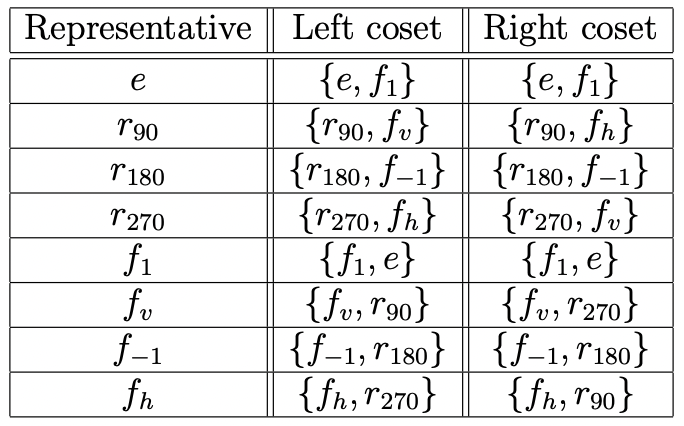
\includegraphics[width=8cm]{coset.png}
	\end{center}
}

\mlenma{}{Let $H<G$, then $H$ is a subgroup of $G$ and let $g_1,g_2$ be arbitrary elements of $G$. Then the following are equivalent:
\begin{enumerate}
	\item $g_1H = g_2H$
	\item $Hg_1^{-1} = Hg_2^{-1}$
	\item $g_1H \subset g_2H$
	\item $g_1 \in g_2H$
	\item $g_1^{-1}g_2 \in H$
\end{enumerate}}

\mpf{Proof}{We will prove that $1 \Longrightarrow 2 \Longrightarrow 3 \Longrightarrow 4 \Longrightarrow 5 \Longrightarrow 1$ so that the statements prove each other in a circular manner, so if any is true the rest become true.

$(1 \Longrightarrow 2)$ Consider a typical element $h g_1^{-1}$ of $H g_1^{-1}$. Its inverse is $g_1 h^{-1}$. Since $h \in H$ and $H$ is a subgroup, $h^{-1} \in H$, so $g_1 h^{-1} \in g_1 H$. Thus it is also in $g_2 H$, so can be written in the form $g_2 h^{\prime}$. So we have $\left(h g_1^{-1}\right)^{-1}=g_2 h^{\prime}$. Take the inverse on both sides, to find $h g_1^{-1}=h^{-1} g_2^{-1}$. Since $h^{\prime} \in H$ we also have $h^{\prime-1} \in H$, so this is a member of $H g_2^{-1}$. In other words, any member of $H g_1^{-1}$ is in $H g_2^{-1}$. The reverse inclusion is proven the same way, so the two sets must be equal to each other.

$(2 \Longrightarrow 3)$ Consider a typical element $g_1 h$ of $g_1 H$. Its inverse is $h^{-1} g_1^{-1} \in H g_1^{-1}=H g_2^{-1}$. So the inverse can be written as $h^{\prime} g_2^{-1}$. Then, reinverting both of these, $g_1 h=g_2 h^{\prime-1} \in g_2 H$. 

$(3 \Longrightarrow 4)$ Since $H$ is a subgroup, $e \in H$, so $g_1 e=g_1 \in g_1 H$. By subsets, it must be in $g_2 H$. 

$(4 \Longrightarrow 5)$ Since $g_1 \in g_2 H$ we know that we can write $g_1=g_2 h$. Rearranging this gives $g_1^{-1} g_2 h=e$ or $g_1^{-1} g_2=h^{-1}$. Since $H$ is a subgroups and $h \in H$, of course $h^{-1} \in H$.

$(5 \Longrightarrow 1)$ Let $g_2 h \in g_2 H$ be a typical element. Since $g_1^{-1} g_2 \in H$ we can choose $k \in H$ so that $g_1^{-1} g_2=k$. Then $g_1^{-1} g_2 h=k h$, or $g_2 h=g_1(k h) . H$ is a subgroup so contains product of its elements, and thus $g_1(k h) \in g_1 H$. Thus any element of $g_2 H$ is in $g_1 H$, or $g_2 H \subset g_1 H$.
Since $g_1^{-1} g_2$ is in $H$, so is its inverse $g_2^{-1} g_1$ so the argument of the previous paragraph may be repeated to show $g_1 H \subset g_2 H$.}

\thm{}{Left cosets $g_1H$ and $g_2H$ are either identical or disjoint. Also true for right cosets.}

\mpf{Proof}{Let $x \in g_1H \cap g_2H$. Then $x \in g_1H$ so therefore $xH = g_1H$. Same argument for $xH = g_2H$. }

\mlenma{}{There is a one-to-one correspondence between left and right cosets.}

\mpf{Proof}{Consider the map $gH \to Hg^{-1}$. It is a well-defined map by statements 1 and 2 of the lemma which also show why this map is one-to-one and onto.}

\nt{$xH = yH \not\Leftrightarrow Hx = Hy$}

\dfn{Index}{The number of cosets of H in G (right or left, since these numbers are the same by the lemma) is called the index of $H$ in $G$ and is denoted by $[G:H]$.}

\mlenma{}{The function $f_g :H \to gH$ given by $f_g(x) = gx$ is a bijection between the elements of $H$ and the elements of $gH$.}

\thm{Lagrange's Theorem}{If $G$ is a finite group and $H$ is a subgroup of $G$, then the following equation is satisfied: $$|G| = [G : H] |H|.$$ }

\mpf{Proof}{Cosets are equinumerous with $H$ and either identical or disjoint, we're done!}

\cor{}{$|H|$ divides $|G|$. }

\cor{}{Groups of prime order are necessarily cyclic, and each non-identity elements are the generators.}

\thm{}{Let $K<H<G$. Then $K < G$, and $[G:K] = [G:H][H:K]$.}

\thm{}{If you have an abelian group $G$ whose order is the product $mn$ where $m$ and $n$ are relativity prime, then $G$ is cyclic. Its generator is $ab$ where $a$ is an element with order $m$ and $b$ is an element with order $n$. }

\thm{Euler}{If $a$ is relatively prime to $n$, then $a^{\phi(n)} \equiv 1 \pmod{n}.$}

\mpf{Proof}{$|U(n)| = \phi(n)$ so the order of every element is a divisor of $\phi(n)$.}

\thm{Fermat's Little Theorem}{If $p$ is a prime number, then $a^p \equiv a \pmod{p}$.}

\mpf{Proof}{If $p$ is a divisor of $a$ then both sides are congruent to zero modulo $p$. Otherwise $\phi(p) = p-1$ and the result obtains by multiplying both sides of the result of Euler's Theorem by $a$.}

\nt{While Lagrange eliminates subgroups of certain orders (order that is relatively prime to the order of the parent group), it does not guarantee the existence of any order. }

\ex{$A_4$}{$A_4$ has 12 elements, but does not have any subgroups of size six. For assume there were such a subgroup $H$. Now $H$ would have only two left cosets-itself and $g H$ for some $g$ not in $H$. But it also only has two right cosets. Since cosets are either disjoint or identical, the right coset of $H$ other then $H$ itself must also be the left coset. That is, $g H=H g$. So for any $h \in H$, there is an $h^{\prime}$ so that $g h=h^{\prime} g$. Another way of saying this is that $g h g^{-1}=h^{\prime} \in H$ for any $h \in H$ and any $g \in G$.

Now consider the three-cycles in $A_4$. There are eight of them. So by the pigeonhole principle, there must be a three-cycle in $H$. Without loss of generality assume $(123) \in H$. By the result of the previous paragraph, $(124)(123)(142)=(243) \in H$. Also, (234) $(123)(243)=$ $(134) \in H$. In fact, all three-cycles must be in $H$. But then $H$ has more than just six elements!}

\thm{}{If $\sigma \in S_n$ is a cycle of length $k$, then $\tau \in S_n$ is also a cycle of length $k$ iff $\tau = g\sigma g^{-1}$ for some $g \in S_n$. }

\cor{}{Two permutations have the same cycle structure if and only if they are conjugates.}

\section{Group Theory}
\subsection{Isomorphisms}
\dfn{Isomorphic}{Let $(G, \cdot)$ and $(H, \circ)$ be groups. We say that $G$ and $H$ are isomorphic if there is a bijection $f:G \to H$ such that $f(g_1 \cdot g_2) = f(g_1) \circ f(g_2)$ for all $g_1, g_2 \in G$.}

\ex{}{$\phi: \ZZ_4 \to \{i, -1, -i, 1\}$ defined by $\phi(n) = i^n$. This is obviously a one-to-one and onto mapping, and trades addition in $\ZZ_4$ for multiplication in $\CC$. }

\thm{}{If $\phi$ is an isomorphism, then so is $\phi^{-1}$.}

\cor{}{If $\phi: G \to H$ is an isomorphism, then:
\begin{itemize}
	\item $\phi(e_G) = e_H$
	\item $\phi(g^{-1}) = \phi(g)^{-1}$
	\item $\phi(g^k) = (\phi(g))^k$
\end{itemize}}

\thm{Cayley's Theorem}{Every group is isomorphic to a permutation group.}

\dfn{Direct Product}{Let $(G, \cdot, e)$ and $(H, \circ, i)$ be groups. The \emph{direct product} of $G$ and $H$, denoted as $G \times H$, is the group whose elements take the form $(g, h)$ for $g \in G$ and $h \in H$. The operation is defined as $(g_1, h_1)(g_2, h_2) = (g_1 \cdot g_2, h_1 \circ h_2)$. The identity element is $(e, i)$.}

\mlenma{}{If $g$ has order $m$ in $G$ and $h$ has order $n$ in $H$, then $(g, h)$ has order lcm($m,n$) in $G \times H$.}

\cor{}{If $m$ and $n$ are relatively prime, then $\ZZ_m \times \ZZ_n$ is isomorphic to $\ZZ_{mn}$.}

\dfn{Internal Direct Product}{Let $G$ be a group with subgroups $H$ and $K$ that fit together as follows:
\begin{itemize}
	\item $H \cap K = \{e\}$
	\item $G = HK = \{hk : h \in H, k \in K\}$
	\item $hk = kh$ for any $h \in H$ and $k \in K$
\end{itemize}
Then $G$ is called the \emph{internal direct product} of $H$ and $K$, and is isomorphic to $H \times K$.
}

\dfn{Normal Subgroup}{A subgroup $H$ of $G$ is called \emph{normal} if $gH = Hg$ for all $g \in G$. }

\thm{}{Let $H$ be a subgroup of $G$. Then the following assertions are equivalent:

\begin{enumerate}
	\item $H$ is normal in $G$.
	\item For any $g \in G$, $gHg^{-1} \subset H$.
	\item For any $g \in G$, $gHg^{-1} = H$.
\end{enumerate}}

\thm{}{Let $N$ be a normal subgroup of $G$. Then the cosets of $N$ form a group denoted $G/N$.}

\ex{$D_5 / R$}{The quotient group $D_5/R = \{\text{rotations}, \text{reflections}\}$. }

\ex{$\ZZ / 8\ZZ$}{$\ZZ / 8\ZZ = \ZZ_8$}

\ex{$D_6$ with the 120 degree rotations}{If we have $N = \{e, r_{120}, r_{240}\}$, then $N$ is normal so we can analyze $D_6 / N$, which we see is the same as $V$. }

\thm{}{If $N$ is normal in $G$ and $H < G$, then $H \cap N$ is normal in $H$. }

\mpf{Proof}{Need to show that for all $h 
in H, hK = Kh$ if we call $K = H \cap N$. Or $hKh^{-1} \subset K$. First we claim that $hkh^{-1} \in H$ because all the elements are in $H$ and groups are closed. Then we claim that $hkh^{-1} \in K$ because $k \in N$, so $hkh^{-1} \in N$ because $N$ is normal in $G$. So, $hkh^{-1} \in H \cap N$.}

\dfn{Simple}{A group with no proper normal subgroups is called \emph{simple}.}

\mlenma{}{All even permutations can be written as a product of 3-cycles ($n\geq 4$).}

\mpf{Proof}{Even permutations are generated by products of even numbers of transpostions. Two transpositions overlap at either 0, 1 or both places. In any case, you can factor it into a product of 3-cycles.}

\mlenma{}{If a normal subgroup of $A_n$, $n\geq 3$, contains even one 3-cycle, then it contains all of $A_n$.}

\mpf{Proof}{If you have $(a \; b \; c)$ and you conjugate it with $(a \; b \; d)$, then you get $(a ;\; c \; d)$. In other words, the conjugate of any 3-cycle forms all 3-cycles, which generate $A_n$.}

\thm{}{For $n \geq 5$, $A_n$ is simple.}

\mpf{Proof}{Let $N$ be a nontrivial normal subgroup of $A_n$. We will show that $N$ contains a three-cycle $\Rightarrow$ is all of $A_n$. Now we check the five cases:
\begin{enumerate}
	\item If $N$ contains a three-cycle, then we're done by previous lemmas.
	\item $N$ contains a permutation $\sigma$ that can be written in cycle notation as $\mu \rho$ where $\rho$ is a cycle whose length is greater than three, say $\rho=\left(a_1 a_2 a_3 a_4 \ldots a_k\right)$. Then by normality, $N$ also contains the permutation $\left(a_1 a_2 a_3\right) \sigma\left(a_3 a_2 a_1\right)$. Since none of the cycles in $\mu$ contain $a_1, a_2$, or $a_3$, we get that $\left(a_1 a_2 a_3\right) \sigma\left(a_3 a_2 a_1\right)=\left(a_1 a_2 a_3\right) \mu \rho\left(a_3 a_2 a_1\right)=$ $\mu\left(a_1 a_2 a_3\right) \rho\left(a_3 a_2 a_1\right)=\mu\left(a_2 a_3 a_1 a_4 \ldots a_k\right)$. Since this is in $N$ and $\sigma^{-1}$ must be in $N$, we can multiply the two to find that $\left(a_k \ldots a_3 a_2 a_1 \right) \mu^{-1} \mu\left(a_2 a_3 a_1 a_4 \ldots a_k\right)=$ $\left(a_k \ldots a_3 a_2 a_1\right)\left(a_2 a_3 a_1 a_4 \ldots a_k\right)=\left(a_1 a_3 a_k\right)$ is in $N-$ so $N$ contains a three-cycle!
	\item $N$ contains a permutation which has all transpositions and three-cycles, containing at least two three-cycles. So $N$ contains an element like $\sigma=\mu\left(a_1 a_2 a_3\right)\left(\begin{array}{lll}a_4 & a_5 & a_6\end{array}\right)$ (note that $n \geq 6$ in this case). $N$ contains $\sigma$ conjugated by $\left(a_1 a_2 a_4\right)$, which is $\mu\left(a_1 a_5 a_6\right)\left(a_2 a_4 a_3\right)$. Multiply this on the left by $\sigma^{-1}$ to find that $N$ also contains $\left(\begin{array}{lll}a_6 & a_5 & a_4\end{array}\right)\left(a_3 a_2 a_1\right)\left(a_1 a_5 a_6\right)\left(\begin{array}{lll}a_2 & a_4 & a_3\end{array}\right)=\left(\begin{array}{lllll}a_1 & a_4 & a_2 & a_6 & a_3\end{array}\right)$ which is a 5-cycle, and we are complete under Case 2.
	
	\item $N$ contains a permutation which has all transpotions and just one three cycle: $\mu\left(a_1 a_2 a_3\right)$. Then $N$ also contains the square of this element, which is $\left(a_1 a_3 a_2\right)$, a three-cycle, so we're done once again.
	
	\item $N$ contains an element that is a product of an even number of transpositions and no other cycles. So $N$ contains an element like $\mu\left(a_1 a_2\right)\left(a_3 a_4\right)$. Conjugate by $\left(a_1 a_2 a_3\right)$ to obtain $\mu\left(a_1 a_4\right)\left(a_2 a_3\right)$. Now multiply this by $\sigma^{-1}$ to obtain $\left(a_1 a_2\right)\left(a_3 a_4\right)\left(a_1 a_4\right)\left(a_2 a_3\right)=$ $\left(a_1 a_3\right)\left(a_2 a_4\right)$. We finally use the fact that $n \geq 5$ to conjugate this by $\left(a_1 a_2 a_5\right)$ yielding $\left(a_2 a_3\right)\left(a_4 a_5\right)$ is also in $N$. Then $N$ contains the product of these last two elements, which is $\left(a_1 a_3 a_4 a_5 a_2\right)$. Since this is a 5 -cycle, we are done by Case 2.
\end{enumerate}}

\dfn{Homomorphism}{Let $(G, \cdot)$ and $(H, *)$ be groups. A \emph{homomorphism} from $G$ to $H$ is a map $\phi: G \to H$ that satisfies $\phi(g\cdot h)=\phi(g)* \phi(h)$ for all $g,h \in G$.}

\ex{Determinants}{The function $\text{det} : GL_n(\RR) \to \RR^*$ is a homomorphism because of the multiplicative property of determinants.}

\ex{Projection Homomorphisms}{Let $G, H$ be any two groups. Then there are two \emph{projection homormorphisms}. Namely, they are $\pi_1(g,h) = g$ and $\pi_2(g,h) = h$ for all $g,h \in G \times H$.}

\ex{Inclusion Homomorphism}{We say that $D_4$ is included in $S_4$ because any symmetry of a square is definitely a permutation of its vertices.}

\ex{Canonical Map}{Let $N \trianglelefteq G$. Then, the \emph{natural map}(or \emph{canonical map}) is the homomorphism $\phi: G \to G/N$ given by $\phi(g) = gN$. }

\nt{\begin{itemize}
	\item An onto map is called a \emph{surjection}.
	\item A one-to-one map is called an \emph{injection}.
	\item A surjective homomorphism is called a \emph{epimorphism}.
	\item An injective homomorphism is called a \emph{monomorphism}.
\end{itemize}}

\thm{}{Let $\phi : G_1 \to G_2$ be a homomorphism. 
\begin{enumerate}
	\item $\phi(e_1) = e_2$.
	\item For $g \in G_1$, $\phi(g^{-1}) = (\phi(g))^{-1}$.
	\item If $H < G$, then $\phi(H) < G_2$. If $H \trianglelefteq G_1$, then $\phi(H)$ is normal in $\phi(G_1)$.
	\item If $H_2 < G_2$, then $\phi^{-1}(H_2) < G_1$. If $H_2 \trianglelefteq G_2$, then $\phi^{-1}(H_2)$ is normal in $\phi^{-1}(G_1)$.
\end{enumerate}}

\dfn{Kernel}{Given a homomorphism $\phi: G_1 \to G_2$. Then, $\{e_2\}$ is normal in $G_2$. By the previous theorem, $\phi^{-1}(\{e_2\})$ is normal in $G_1$. The inverse image is called the \emph{kernel} of $\phi$.}

\thm{First Isomorphism Theorem}{Let $\varphi: G \to H$ be a homomorphism of $G$ onto $H$. Let $K$ be the kernel of $\varphi$ and let $\phi: G \to G/K$ be the natural homomorphism. Then there is a unique isomorphism $\psi: G/K \to H$ such that $\psi \circ \phi = \varphi$.}

\thm{Second Isomorphism Theorem}{Let $G$ be a group, $H$ a subgroup, and $N$ a normal subgroup. Then $H \cap N$ is normal in $H$, $HN$ is normal in $N$, and $H/(H \cap N)$ is isomorphic to $HN/N$.}

\thm{Third Isomorphism Theorem}{Let $G$ be a group with normal subgroups $H$ and $N$ with $N \subset H$. Then $G/H \cong \displaystyle \frac{G/N}{H/N}$. }

\thm{Correspondence Theorem}{If $H_1$ and $H_2$ are subgroups of $G$ that contain $N$, then 
\begin{enumerate}
	\item $A \subset B$ iff $A/N \subset B/N$.
	\item If $A \subset B$, then $[B:A] = [B/N:A/N]$.
	\item $\langle A, B \rangle/N = \langle A/N, B/N \rangle$.
	\item $(A \cap B)/N  = (A/N) \cap (B/N)$.
\end{enumerate}}

\thm{Fundmental Theorem of Finite Abelian Groups}{Every finite abelian group $G$ is isomorphic to a direct product of cyclic groups $\ZZ_a$ where $a$ is a prime power.}

\thm{}{Given a non-trivial abelian group, the following two conditions are equivalent for a subset $X$ of $G$.
\begin{enumerate}
	\item Every non-zero element $x \in G$ can be expressed as a linear combination of $x_i$. 
	\item $X$ generates $G$ and no linear combination equals 0 for nonzero coefficients.
\end{enumerate}}

\dfn{Free Abelian Group}{A group $G$ that has a subset that generates $G$ where the only relation is $ab=ba$ is called a \emph{free abelian group}.}

\thm{}{If $G$ is a free abelian group with finite bases, then all bases for $G$ are finite with the same number of elements.}

\section{Counting}
\dfn{Rank}{The \emph{rank} of a free abelian group with a finite basis is the number of elements in a basis.}

\dfn{G-equivalent}{$x \sim_G y$ if $y = gx$ for some $g \in G$ and $x,y \in X$.}

\dfn{Orbit}{The \emph{orbit}, $O_x$ is all $y$ such that $x \sim_G y$.}

\dfn{Fixed-point set}{Let $G$ act on $X$. Choose a particular element $g \in G$. The set $X_g = \{x \in X : gx = x\}$ is called the \emph{fixed-point set} of $g$. }

\dfn{Stabilizer}{Let $G$ act on $X$. Choose a particular element $x \in X$. The set $G_x = \{g \in G : gx = x\}$ is called the \emph{stabilizer} of $x$. }

\mlenma{}{The stabilizer of any element of $X$ is a subgroup of $G$.}

\mpf{Proof}{The proof is by direct computation. The stabilizer is also called the stabilizer subgroup, or sometimes the \emph{isotropy} group.}

\thm{}{For any finite group $G$ and finite $G$-set $X$, given $x \in X$, then $|O_x| = [G:G_x]$.}

\dfn{$X_G$}{$X_G = \{x \in X : gx =x \forall g \in G\}$}

\nt{If $x \in X_G$, then $|O_x| = 1$. Thie yields us a simple equation for the order of $X$:
$$|X| = |X_G| + \sum_{i=1}^{k}|O_{x_i}|$$}

\dfn{Class Equation}{$$|G| = |Z(G)| + \sum_{i=1}^k[G:C(x_i)]$$}

\cor{}{The order of any conjugacy class must divide the order of the group.}

\cor{}{A group of order $p^n$ where $p$ is prime has a nontrivial center.}

\thm{Cauchy's Theorem}{If $p$ is prime and divides $|G|$, then $G$ has a subgroup of order $p$.}

\mlenma{}{Let $X$ be a $G$-set and $x \sim_G y$. Then $G_x$ and $G_y$ are isomorphic.}

\thm{Burnside's Theorem}{Let $G$ be a finite group and $X$ a finite $G$-set. If $k$ is the number of orbits of $G$, then
$$k = \frac{1}{|G|}\sum_{g \in G}|X_g|.$$ }

\mpf{Proof}{First we have to understand that the following equation:
$$\sum_{g \in G}|X_g| = \sum_{x \in X}|G_x|$$

Both of these go through all the elements of $X$ and count each one a number of times equal to the number of elements of $G$ that fix it, so these sums must be equal.

Now, within any orbit, all the $|G_y|$ for $y$ in that orbit are equal (all such stabilizers are isomorphic, so trivially they are equinumerous). So for each orbit $\mathcal{O}_x$, the portion of the sum relating to it is given as follows:
$$\sum_{y \in \mathcal{O}_x}|G_y| = |\mathcal{O}_x||G_x|.$$

Now we know that $|\mathcal{O}_x| = [G : G_x] = |G|/|G_x|$. So each orbit contributes $|G|$ to the sum of $\sum_{x \in X}|G_x|$. Since there are $k$ orbits, the final sum must be $k|G|$, and the theorem follows.
}

\section{Rings}
\dfn{Ring}{A \emph{ring} is a set $R$ with two binary operations and is denoted as $(R, +, \cdot)$, that satisfies the following conditions:
\begin{itemize}
	\item $(R, +)$ is an abelian group.
	\item $(R, \cdot)$ is associative.
	\item $\cdot$ distributes over $+$.
\end{itemize}}

\mlenma{}{If $R$ is a ring, then 
\begin{itemize}
	\item $0x = x0 = 0$ for all $x \in R$
	\item $(x)(-y) = (-a)(b) = -(ab)$ for all $a,b \in R$
	\item $(-a)(-b) = ab$ for all $a,b \in R$
\end{itemize}}
\mpf{Proof}{Note that $a0 = a(0 + 0) = a0 +a0$ and the result is obtained by additive cancellation.

The same works for $0a = (0 + 0)a = 0a + 0a$.

Then $0 = a0 = a(b+ (-b)) = ab+a(-b)$. Adding the opposite $-(ab)$ to both sides yields $a(-b) = -(ab)$. The other half is similar using $0b = (a + (-a))b$.

The third bullet comes from the second and the fact that the inverse of the inverse is the original element by uniqueness of inverses.}

\dfn{Ring with unity}{If a ring has a multiplicative identity (which will usually be notated 1, though
note that matrices often use I for the identity), it is called a \emph{ring with unity}.}

\dfn{Unit}{In a ring with unity, any element with an inverse is called  an \emph{unit}.}

\dfn{Division Ring}{A ring with unity in which each non-zero element is a unit is called a \emph{division ring} (or a \emph{skew field}).}

\dfn{Field}{A commutative division ring is called a \emph{field}.}

\dfn{Zero Divisor}{In any ring, non-zero elements $a$ and $b$ are called \emph{zero divisors} if $ab = 0$. $a$ is the left zero divisor while $b$ is the right zero divisor.}

\mlenma{Left Cancellation}{If $a$ is not a left zero divisor and $ab=ac$, then $b=c$. }
\mlenma{Right Cancellation}{If $a$ is not a right zero divisor and $ba=ca$, then $b=c$. }

\dfn{Integral Domain}{A commutative ring with no zero divisors is called an integral domain.}

% \section{Random Examples}
% \begin{myproof}By openness of $V$, $x\in B_r(u)\subset V$
% 	\begin{center}
% 		\begin{tikzpicture}
% 			\draw[red] (0,0) circle [x radius=3.5cm, y radius=2cm] ;
% 			\draw (3,1.6) node[red]{$V$};
% 			\draw [blue] (1,0) circle (1.45cm) ;
% 			\filldraw[blue] (1,0) circle (1pt) node[anchor=north]{$u$};
% 			\draw (2.9,0.4) node[blue]{$B_r(u)$};
% 			\draw [green!40!black] (1.7,0) circle (0.5cm) node [yshift=0.7cm]{$B_{\delta}(x)$} ;
% 			\filldraw[green!40!black] (1.7,0) circle (1pt) node[anchor=west]{$x$};
% 		\end{tikzpicture}
% 	\end{center}
% \end{myproof}

% \cor{}{By the result of the proof, we can then show...}

% \mprop{}{$1 + 1 = 2$.}

% \section{Random}
% \dfn{Normed Linear Space and Norm $\boldsymbol{\|\cdot\|}$}{Let $V$ be a vector space over $\bbR$ (or $\bbC$). A norm on $V$ is function $\|\cdot\|\ V\to \bbR_{\geq 0}$ satisfying \begin{enumerate}[label=\bfseries\tiny\protect\circled{\small\arabic*}]
% 		\item \label{n:1}$\|x\|=0 \iff x=0$ $\forall$ $x\in V$
% 		\item \label{n:2}	$\|\lambda x\|=|\lambda|\|x\|$ $\forall$ $\lambda\in\bbR$(or $\bbC$), $x\in V$
% 		\item \label{n:3} $\|x+y\| \leq \|x\|+\|y\|$ $\forall$ $x,y\in V$ (Triangle Inequality/Subadditivity)
% 	\end{enumerate}And $V$ is called a normed linear space.

% 	$\bullet $ Same definition works with $V$ a vector space over $\bbC$ (again $\|\cdot\|\to\bbR_{\geq 0}$) where \ref{n:2} becomes $\|\lambda x\|=|\lambda|\|x\|$ $\forall$ $\lambda\in\bbC$, $x\in V$, where for $\lambda=a+ib$, $|\lambda|=\sqrt{a^2+b^2}$ }


% \section{Algorithms}
% \begin{algorithm}[H]
% \KwIn{This is some input}
% \KwOut{This is some output}
% \SetAlgoLined
% \SetNoFillComment
% \tcc{This is a comment}
% \vspace{3mm}
% some code here\;
% $x \leftarrow 0$\;
% $y \leftarrow 0$\;
% \uIf{$ x > 5$} {
%     x is greater than 5 \tcp*{This is also a comment}
% }
% \Else {
%     x is less than or equal to 5\;
% }
% \ForEach{y in 0..5} {
%     $y \leftarrow y + 1$\;
% }
% \For{$y$ in $0..5$} {
%     $y \leftarrow y - 1$\;
% }
% \While{$x > 5$} {
%     $x \leftarrow x - 1$\;
% }
% \Return Return something here\;
% \caption{what}
% \end{algorithm}

\end{document}